\section{Backend}
\begin{center}
    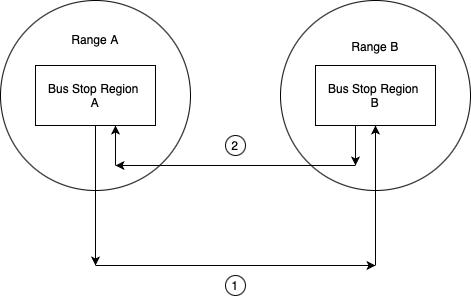
\includegraphics[scale = 0.75]{Files/Images/Img1.jpeg}
\end{center}
We define the following notations : 
\begin{align*}
    T_{AB} &:= A\to B \text{ along path $1$} \\
    T_{BA} &:= B\to A \text{ along path $2$}
\end{align*}
\noindent If the bus stops within the \textsc{BusStopRegion-A}, we update the timer of $A$ to $0$ and update the timer of $B$ to $T_{AB}$ when the bus moves again. If the bus stops within the range of $A$ but outside the bus stop region, we paus the timer for both $A$ and $B$ and resume it when the bus moves again.

\noindent\textbf{Proof}
\begin{center}
    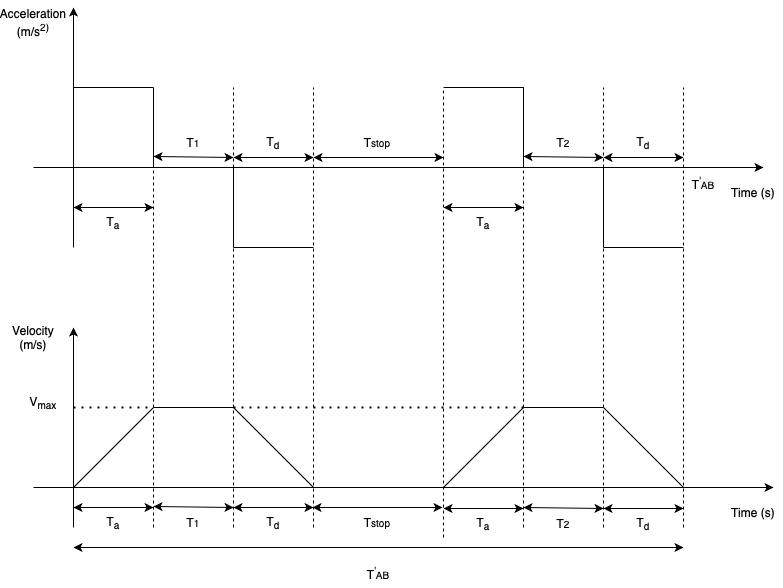
\includegraphics[scale = 0.5]{Files/Images/Img2.jpeg}
\end{center}
We assume that the bus has a fixed acceleration/deceleration profile whenever bus moves and bus moves at $v_{\max}$ from $t_0$ (when bus doesn't stop in between).
\begin{center}
    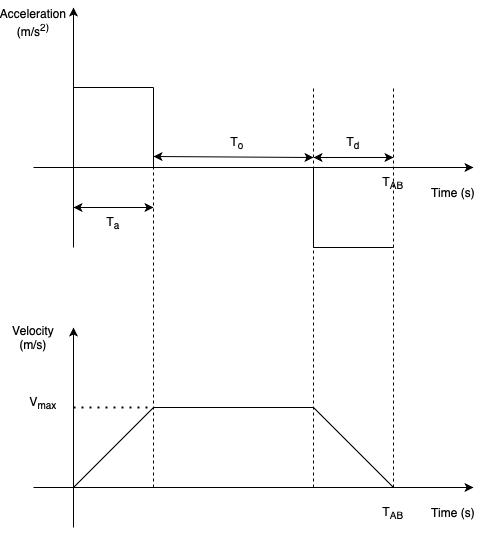
\includegraphics[scale = 0.5]{Files/Images/Img3.jpeg}
\end{center}

Note that : 
\begin{gather*}
    T_{AB}= t_{a}+t_0 + t_d \\
    T_{AB}' = 2t_{a}+2t_d + t_1+t_2 + T_{\operatorname{stop}} \tag{1}
\end{gather*}

\noindent Since the distance covered is the same, the area under the curves should also be the same. Writing out the expressions for the areas, we get : 
\[\frac12 v_{\max}\cdot T_{AB} = \frac12 v_{\max} (t_a + t_1 + t_d) + \frac12 v_{\max} (t_a+t_2+t_d).\]
Hence, it follows that : 
\[T_{AB} = 2t_a + 2t_d + t_1 + t_2\tag{2}\]
Combining $(1)$ and $(2)$, we get :
\[T_{AB}' = T_{AB} + tT_{\operatorname{stop}}\]
Hence, pausing the timer as soon as the bus is halted, does the job.